\documentclass{article}
\usepackage{graphicx} % Required for inserting images
\usepackage[T1]{fontenc}
\usepackage[polish]{babel}
\usepackage[utf8]{inputenc}
\usepackage{amssymb}
\usepackage{tikz}
\usepackage{amsmath}
\usepackage{listings}
\usepackage{graphicx}
\usepackage[a4paper, left=40mm, right=40mm, top=30mm, bottom=30mm]{geometry}
\usepackage[indent=0pt]{parskip}

\graphicspath{ {./charts/} }
\usepackage{csquotes}

\title{Sortowanie plików sekwencyjnych metodą scalania naturalnego}
\author{Jerzy Szyjut}
\date{26.11.2024}

\begin{document}

\maketitle

\section{Wybór implementacji}
W ramach mojego projektu zaimplementowałem metodę scalania naturalnego na trzech taśmach w schemacie 2+1. Jako typ rekordu wylosowałem 5 liczb, które są sortowane po średniej arytmetycznej, liczby zapisywane są w 4-bajtowym typie int. Program zaimplementowałem w języku C++. 

\section{Wprowadzenie teoretyczne}
\subsection{Wstęp}
Sortowanie przez scalanie składa się z faz, na każdą z faz składają się dwa etapy, etap rozdziału i etap scalania. Etapy te po kolei zmniejszają liczbę serii, czyli niemalejących ciągów liczb. Algorytm ten z każdą fazą zmniejsza liczbę serii (i zwiększa ich długość), aż skończy na jednej serii o długości całego pliku. 

Stałe używane później w sprawozdaniu:
\begin{itemize}
\item $N$ - liczba rekordów w pliku
\item $B$ - rozmiar bloku w bajtach
\item $R$ - rozmiar rekordu w bajtach
\item $r$ - liczba serii występujących w pliku
\item $b = B/R$ - liczba rekordów na blok
\end{itemize}

\subsection{Rozdzielanie}
W etapie rozdzielania, rozdzielamy serie z jednej taśmy (na początku tą taśmą jest plik wejściowy) na dwie taśmy. Robimy to w ten sposób
\begin{enumerate}
    \item Przenosimy liczby na pierwszą z dwóch taśm
    \item Napotykamy koniec serii, następne liczby przenosimy na drugą z dwóch taśm
    \item Napotykamy koniec serii, wracamy do przenoszenia liczb na pierwszą z taśm
    \item Robimy tak, aż nie wyczerpiemy liczb na pierwszej z taśm
\end{enumerate}
Przykładowo (znaki $|$ są tylko, aby podkreślic, gdzie kończą się serie):

Taśma wejściowa - $[$$46$ $59$ $77$ $|$ $55$ $75$ $|$ $44$ $57$ $|$ $73$ $]$

Wedle algorytmu rozdzielamy liczby na dwie taśmy zmieniając taśmy po napotkaniu końca serii

1.

T1 - $[$ $46$ $59$ $77$ $]$

T2 - $[]$


2.

T1 - $[$ $46$ $59$ $77$ $]$

T2 - $[$ $55$ $75$ $]$


3.

T1 - $[$ $46$ $59$ $77$ $|$ $44$ $57$ $]$

T2 - $[$ $55$ $75$ $]$

4.

T1 - $[$ $46$ $59$ $77$ $|$ $44$ $57$ $]$

T2 - $[$ $55$ $75$ $|$ $73$ $]$

\subsection{Scalanie}
W etapie rozdzielania, scalamy serie z dwóch taśm na jedną. W tym etapi zmniejszamy liczbę serii i je wydłużamy. Algorytm scalania jest bardzo podobny do tego z algorytmu merge sort. Scalamy pierwszą serię taśmy pierwszej z pierwszą serią taśmy drugiej, później drugą z drugą itd. W przypadku, gdy na drugiej taśmie nie ma odpowiadającej serii, dopełniamy taśmę tą "samotną" serią.

Przykładowo (znaki $|$ są tylko, aby podkreślic, gdzie kończą się serie):

T1 - $[$ $46$ $59$ $77$ $|$ $44$ $57$ $]$

T2 - $[$ $55$ $75$ $|$ $73$ $]$

Taśma wyjściowa - $[$ $46$ $55$ $59$ $75$ $77$ $|$ $44$ $57$ $73$ $]$

\subsection{Analiza}
Algorytm ten pozwala na sortowanie danych o rozmiarach znacznie przekraczających rozmiar pamięci operacyjnej, gdy zastosuje ładowanie danych z i do taśm blokami (na wzór stronnicowania i pamięci wymiany). W wypadku tego algorytmu zużywamy $B$ pamięci RAM i $N \times R$ pamięci dyskowej.  

Liczbę faz potrzebnych do posortowania pliku można obliczyć za pomocą wzoru
$$\lceil \log_2 r \rceil$$

Liczby operacji dyskowej w przypadku pesymistycznym można obliczyć za pomocą wzoru
$$ 4N \lceil \log_2 N \rceil / b$$

Liczby operacji dyskowej w przypadku średnim można obliczyć za pomocą wzoru
$$ 4N \lceil \log_2 r \rceil / b$$

\section{Specyfikacja formatu pliku}
Plik sekwencyjny z danymi jest plikiem binarny i zawiera kolejno rekordy jeden po drugim w 4-bajtowej postaci binarnej reprezentującej liczby. Jeden rekord zawiera dokładnie 20 bajtów. Plik nie zawiera metadanych, nagłówków rekordów czy separatorów. Program odczytuje i zapisuje dane z pliku za pomocą klasy $Tape$. Odczyt z pliku odbywa się w blokach o dowolnej wielkości będącej wielokrotnością rekordu.

\section{Sposób prezentacji wyników działania programu}
Menu wyboru akcji w programie jest wywoływane w momentach kluczowych dla algorytmu (przed uruchomieniem algorytmu, po każdym rozdziale, scalaniu i po posortowaniu pliku). Menu pozwala na nadpisywanie taśm oraz podglądywanie taśm oraz wybór momentów wstrzymywania algorytmu. Po wykonaniu się programu prezentowane są statystyki.

\subsection{Menu}
\begin{lstlisting}
Stopped before sorting
Stopped by debug controller. Available commands:
n - continue
p - print tape
a - add random records to tape
i - add records to tape manually
b - create binary file with numbers
c - change tape to load from specific file
s - stop before sorting (toggle). Currently: on
m - stop after merge (toggle). Currently: off
d - stop after distribute (toggle). Currently: off
o - stop after sort (toggle). Currently: off
q - quit
\end{lstlisting}

\subsection{Wyświetlanie zawartości taśmy}
\begin{lstlisting}
p
Choose tape to print:
1 - input tape
2 - tape 1
3 - tape 2
4 - output tape
q - quit
Choice: 1
Tape: input.dat
Mode: read
Current record index: 0
Records: 
[ 6644 1226 9184 7828 9187  average: 6813.8 ]
[ 8595 4649 6371 6095 7326  average: 6607.2 ]
[ 3420 5301 2729 7611 8681  average: 5548.4 ]
[ 4216 6071 1415 2995 4827  average: 3904.8 ]
[ 5643 8224 5335 9136 4675  average: 6602.6 ]
[ 1599 2547 2773 3394 1692  average: 2401 ]
[ 9271 6197 4500 2670 9359  average: 6399.4 ]
[ 3951 6471 3729 4091 4223  average: 4493 ]
[ 4818 910 3991 3534 7029  average: 4056.4 ]
[ 9118 8922 7107 9058 3331  average: 7507.2 ]
\end{lstlisting}

\subsection{Końcowe statystyki}
\begin{lstlisting}
Number of series: 504
Expected number of phases: 9
Actual number of phases: 8
Expected number of read/write operations: 3600
Actual number of read operations: 1809
Actual number of write operations: 1907
Actual number of read/write operations: 3716
\end{lstlisting}

\section{Eksperyment}
Przy pomocy programu przeprowadziłem eksperymenty losując rekordy przy tym samym ziarnie generatora liczb losowych. Zrobiłem tak dla rozmiarów stron 10, 50 i 100.  Następnie wyniki mojego algorytmu porównałem z oczekiwanymi wynikami wynikającymi ze wzorów.

\begin{center}
\begin{tabular}{ c | c c | c c c c | c c}
 b  & N         & r & odczyty       & zapisy         & o+z       & liczba faz & t. o+z & t. liczba faz\\ 
\hline
 10 & 10        & 4         & 7         & 6         & 13        & 1     & 8         & 2  \\  
 10 & 100       & 44        & 129       & 125       & 254       & 6     & 240       & 6  \\
 10 & 1000      & 505       & 1810      & 1808      & 3618      & 9     & 3600      & 9 \\
 10 & 10000     & 4958      & 26015     & 26011     & 52026     & 13    & 52000     & 13 \\
 10 & 50000     & 24944     & 150020    & 150015    & 300035    & 15    & 300000    & 15 \\
 10 & 100000    & 49983     & 320022    & 320015    & 640037    & 16    & 640000    & 16 \\
 \hline
 50 & 10        & 6         & 10        & 10        & 20        & 3     & 2        & 3  \\  
 50 & 100       & 50        & 37       & 35       & 72       & 6     & 58       & 6  \\
 50 & 1000      & 519       & 371      & 369      & 740      & 9     & 800      & 10 \\
 50 & 10000     & 4948      & 5216     & 5213     & 10429     & 13    & 10429     & 13 \\
 50 & 50000     & 25018     & 30021    & 30015    & 60036    & 15    & 60000    & 15 \\
 50 & 100000    & 49996     & 64037    & 64032    & 128069    & 16    & 128000    & 16 \\
  \hline
 100 & 10        & 3         & 7         & 7         & 14        & 2     & 0        & 2  \\  
 100 & 100       & 51        & 23       & 21       & 44       & 6     & 24       & 6  \\
 100 & 1000      & 484       & 191      & 189      & 380      & 9     & 360      & 9 \\
 100 & 10000     & 5014      & 2613     & 2613     & 5230     & 13    & 5200     & 13 \\
 100 & 50000     & 24930     & 15036    & 15030    & 30066    & 15    & 30000    & 15 \\
 100 & 100000    & 50014     & 32034    & 32029    & 64037    & 16    & 64063    & 16 \\
\end{tabular}

Dla $b=10$

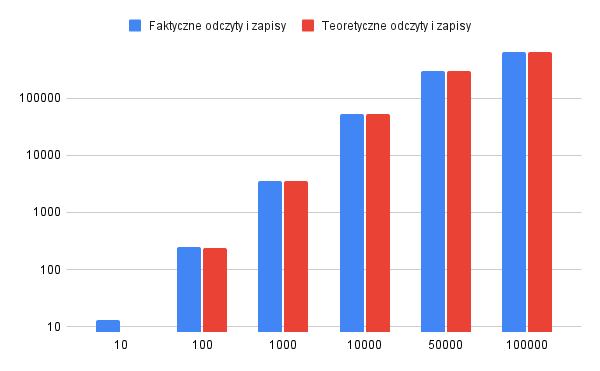
\includegraphics[width=0.8\textwidth]{charts/b_10.png}

Dla $b=50$

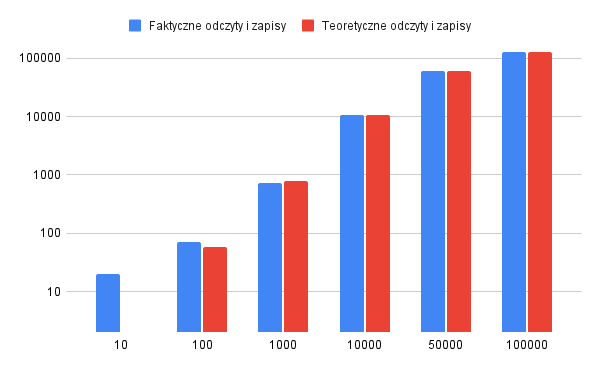
\includegraphics[width=0.8\textwidth]{charts/b_50.png}

Dla $b=100$

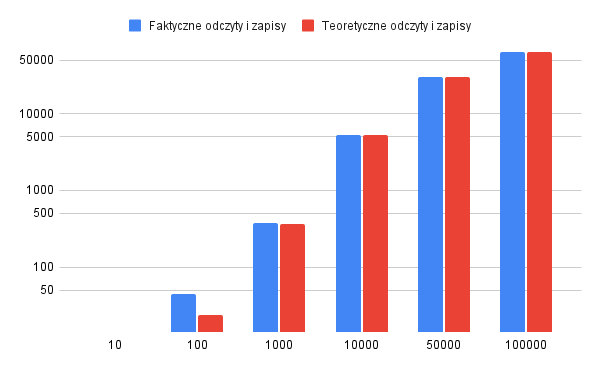
\includegraphics[width=0.8\textwidth]{charts/b_100.png}

Dla $b=10$, $b=50$ i $b=100$ 

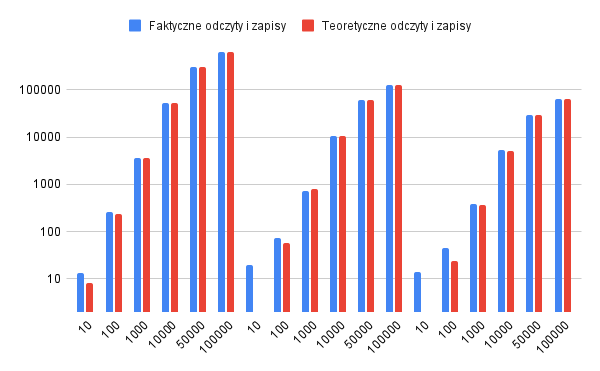
\includegraphics[width=0.8\textwidth]{charts/b_all.png}

\end{center}

Dla danych powyżej widać, że wyniki programu są zbliżone do teoretycznych wyników wyliczonych ze wzorów. Algorytm dokonuje kilku nadmiarowych zapisów i odczytów, ale ich liczba nie wzrasta szybko, ma marginalny narzut na całkowitą liczbę zapisów i odczytów (dla wyższych wyników poniżej $1\%$). Wyniki na wykresach przedstawiłem na skali logarytmicznej, można wywnioskować z nich, że ilość odczytów i zapisów jest zbliżona do zależności liniowej. Liczba faz nie zmienia się w zależności od wielkości bloków, jedynie w zależności od liczby serii i rekordów.  

\section{Wnioski}

Wyniki eksperymentu można uznać za zbliżone do wyników teoretycznych i zgodne z oczekiwaniami, drobne odstępstwa wynikają z szczegółów implementacyjnych algorytmu. Liczba operacji zapisu i odczytu jest odwrotnie proporcjonalna do rozmiaru bloku, a rozmiar bloku nie ma wpływu na liczbę faz.  

\end{document}
